\chapter{RNAs não-codificadores}
\label{sec:ncRNACodificadores}

Neste capítulo descreveremos os RNAs não-codificadores (ncRNAs), que serão objeto de estudo deste trabalho de doutorado. Na seção~\ref{sec:ConBasico}, estudamos ncRNAs de forma geral. Na Seção \ref{sec:ClassNCrnas}, são apresentadas classificações e descrições dos ncRNAs. Em seguida, na Seção~\ref{sec:FerraCompDet}, são descritas algumas ferramentas computacionais para detecção de ncRNAs das classes conhecidas. Na Seção~\ref{sec:bd-ncRNA}, mostraremos os bancos de dados utilizados. Na Seção~\ref{sec:CaracDesafDetec}, seguem características e desafios na detecção de ncRNAs, que serviram de motivaram para esta pesquisa.


\subsection{Conceitos Básicos} \label{sec:ConBasico}

RNA não-codificadores (ncRNA) são tipos específicos de RNA que não codificam proteínas~\citep{watson1953molecular:1953,eddy2001non:2001}, entretanto sua conformação permite que desempenhem funções em vários processos celulares.

O primeiro enunciado do Dogma Central da Biologia Molecular dizia que a função dos RNAs, restringia-se a participação em síntese de proteínas. Contudo, estudos recentes revelam que a quantidade de ncRNAs equivale a 98\% do genoma humano. Uma quantidade tão grande de ncRNAs não pode simplesmente estar sendo produzida sem razão. Portanto atualmente vários estudos  pretendem compreender melhor o papel desses RNAs nos organismos.

	
Apesar de identificados, e possuírem papel de grande importância, a caracterização dos RNAs não-codificadores foi, nas décadas de 1980 e 1990, abandonada e relegada para um segundo plano, talvez devido a dificuldades técnicas relacionadas a identificar essas moléculas pequenas, instáveis e pouco abundantes~\citep{eddy2001non:2001}. Nesta época, os RNAs não envolvidos diretamente com a síntese de proteínas eram chamados de DNA lixo (\textit{junk} DNA)
~\citep{setubal1997introduction:1997}.


	A partir do início dos anos 2000, retomaram-se os estudos dos ncRNAs, em consequência da crescente quantidade de ncRNAs identificados pelos biólogos e descritos na literatura. As descobertas mais notáveis envolvendo RNAs estruturais estão relacionadas ao desenvolvimento do sistema nervoso, corroborando a observação de que a quantidade de regiões não-codificadoras é proporcional à complexidade dos organismos ~\citep{badger1999critica:1999,mattick2001evolution:2001,mercer2008specific:2008,presutti2006non:2006}. Além dos \textit{small interfering} RNA (siRNA) e micro RNAs (miRNA) que ocorrem nos organismos, foram desenvolvidos novos métodos artificiais baseados nos mecanismos nos quais esses RNAs estavam envolvidos, citando principalmente silenciamento de RNAs mensageiros alvo, que já são empregados com sucesso~\citep{reynolds2004rational:2004}.


	Os métodos computacionais para identificar ncRNAs sofrem de problemas similares aos dos métodos experimentais. A Bioinformática não possui métodos únicos para identificação e classificação de ncRNAs, embora alguns critérios sejam usados, como: o fato de que ncRNAs não possuem em geral ORFs longas; há ao longo de sua sequência ocorrências de códons de parada maiores do que a esperada~\citep{wahlestedt2006natural:2006}; provavelmente RNAs tem uma conservação em nível de estrutura secundária e não primária, o que invalida a detecção de ncRNAs por meio de ferramentas tradicionais usadas para caracterizar similaridade de DNA em proteínas \citep{pang2006rapid:2006,rivas2001noncoding:2001,torarinsson2006thousands:2006}. Estudos que incorporam uso de códons, substituições sinônimas e não-sinônimas e energia mínima de dobramento também são bem-sucedidos na identificação de ncRNAs~\citep{badger1999critica:1999,torarinsson2006thousands:2006,xue2005classification:2005}.
	
	Geralmente, os ncRNAs não possuem uma sequência conservada, tendo como principal característica a conservação de sua estrutura espacial que inclui bidimensional ou tridimensional, tornando sua identificação mais difícil. Os ncRNAs mais conhecidos  possuem uma estrutura tridimensional complexa e têm funções tanto catalisadoras como estruturais ~\citep{eddy:2002}. A atual tendência dos métodos de Bioinformática é recorrer a uma combinação de diversos métodos computacionais que caracterizem os ncRNAs por meio de diferentes princípios, e depois analisar todas as informações geradas pelos métodos para decidir quais RNAs provavelmente são
não-codificadores~\citep{mignone2006discrimination:2006,liu:2006}.
	
	
	Sabendo que o problema na busca de ncRNA é essencialmente de classificação,  a escolha de um método depende dos dados disponíveis das sequências que estão sendo analisadas~\citep{rivas2001noncoding:2001,wang2006psol:2006}.  Uma desvantagem é que para confirmar a predição feita \textit{in silico} de um transcrito computacional ser codificador, que exige validação experimental no laboratório, a observação de ausência de tradução não é conclusiva, já que o eventual transcrito poderia ser traduzido logo que exposto a outras condições, ambientais ou fisiológicas~\citep{mignone2006discrimination:2006,liu:2006}.


Desde a descoberta dos ncRNAs, muitas perguntas têm sido feitas e muitos estudos têm sido direcionados à procura de respostas. Porém, essas moléculas ainda não são bem conhecidas. A principal causa disso é que maior parte das pesquisas para detecção de genes, durante muito tempo, foram voltadas na direção de RNAs mensageiros e proteínas.


\subsection{Classificações de ncRNAs} \label{sec:ClassNCrnas}

Os ncRNAs, são classificados, em geral, de acordo com suas funcionalidades, o que permite entender diferentes aspectos relacionados às suas sequências genômicas e, portanto, ao papel que os ncRNAs realizam nos mecanismos celulares. Na Tabela~\ref{fig:ClassncRNAs} são tratadas classes de ncRNAs importantes.

\begin{table}[ht]
 \scalefont{0.8}
 \caption{Alguns tipos de ncRNAs e suas funções conhecidas~\citep{setubal1997introduction:1997,eddy2001non:2001}} \label{fig:ClassncRNAs}\begin{tabular}{|c|l|l|}
\hline
\multicolumn{ 3}{|c|}{\textbf{Classes de ncRNAs}} \\ \hline
\textbf{Sigla} &  \textbf{Função}   & \textbf{Referências} \\ \hline
tRNA &  envolvidos na tradução de mRNAs &~\citep{pavon2009trna:2009}\\ \hline
rRNA &  RNA constituinte do ribossomo &~\citep{eddy2001non:2001} \\ \hline
snoRNA &  envolvidos na modificação do rRNA &~\citep{durbin1998biological:1998}  \\ \hline
miRNA &  família putativa de genes reguladores da tradução. &~\citep{mendell2005micrornas:2005}  \\ \hline
siRNA &  moléculas ativas na interferência de RNA &~\citep{eddy2001non:2001}\\ \hline
piRNA &  regulação de tradução e estabilidade de mRNA, entre outras &~\citep{brennecke2007discrete:2007}  \\ \hline
snRNA &  incluem RNAs relacionados ao processo de excisão &~\citep{stryer:2002}\\ \hline
snmRNA &  essencialmente pequenos RNAs não-codificadores &~\citep{huttenhofer2001rnomics:2001}  \\ \hline
stRNA &  interrompem a tradução de mRNA &~\citep{eddy2001non:2001}  \\ \hline
rasiRNA &  silenciamento da transcrição via remodelagem da cromatina &~\citep{xie2004genetic:2004}  \\ \hline
\end{tabular}
\label{}
\end{table}


O \textbf{RNA transportador (tRNA)}~\citep{pavon2009trna:2009} é utilizado como molécula transportadora de informação de cada códon componente do mRNA em um aminoácido específico a ser adicionado à proteína sendo formada. O tRNA desempenha essa função através de duas regiões, o anticódon que é responsável pelo reconhecimento de códons específicos do mRNA, e o aminoácido correspondente ao códon.

O \textbf{RNA ribossomal (rRNA)}~\citep{eddy2001non:2001} é o componente central do ribossomo. A função do rRNA é prover um mecanismo para decodificar o mRNA em aminoácidos e interagir com os tRNAs durante a tradução, de síntese de proteína.

O \textbf{\textit{small nucleolar} RNA (snoRNA)}~\citep{durbin1998biological:1998} é uma classe de pequenas moléculas que realizam modificações químicas no rRNA, além de outros ncRNAs, tal como o tRNA. Essas modificações possuem como principal objetivo promover a maturação desses ncRNAs, transformando-os em moléculas ativas. A origem desses genes ainda não está clara, mas acredita-se que eles originam-se dos íntrons do mRNA.

O \textbf{microRNA (miRNA)}~\citep{mendell2005micrornas:2005} parece estar relacionado com a regulação gênica. As moléculas de miRNA são parcialmente complementares a uma ou mais moléculas de mRNA e sua principal função é reduzir a expressão de genes codificadores, inibindo a tradução de mRNAs.

\textbf{\textit{small interfering} RNA(siRNA)}~\citep{eddy2001non:2001} possui o mesmo papel do miRNA, porém reduz a expressão de genes codificadores degradando o mRNA em vez de inibir sua tradução.

\textbf{\textit{piwi-interacting} RNA (piRNA)}~\citep{brennecke2007discrete:2007} é uma classe de pequenas moléculas de RNA existentes basicamente nas células de mamíferos. Assim como os miRNAs e os snoRNAs, os piRNAs também estão relacionados com a regulação gênica. Mais especificamente, eles atuam no silenciamento de genes capazes de se auto-duplicar no interior do genoma.

%\textbf{\textit{functional} RNA (fRNA)}~\citep{carter2001computational:2001} é uma molécula que provê a relação entre a tripla do código genético e os aminoácidos codificados


\textbf{\textit{Small nuclear} RNA (snRNA)}~\citep{stryer:2002} é uma classe de RNAs não-codificantes encontrados no interior do núcleo das células. O núcleo contém muitos tipos de snRNAs. A estrutura secundária desses RNAs é altamente conservada nos organismos. Alguns deles, conhecidos como U1, U2, U4, U5 e U6, são essenciais para o \textit{splicing} do pre-mRNA.


\textbf{\textit{small non-messenger} RNA (snmRNA)}~\citep{huttenhofer2001rnomics:2001} é uma classe de ncRNAs, com função reguladora.


\textbf{\textit{Small temporal} RNA (stRNA)}~\citep{eddy2001non:2001} é uma classe de RNAs com função de regulação do desenvolvimento biológico.

\textbf{\textit{repeat-associated} siRNA (rasiRNAs)}~\citep{xie2004genetic:2004} estão envolvidos na manutenção da metilação do DNA e histonas em retrotranposons, são sequências repetitivas como as codificadoras de RNA
ribossomal. A formação de heterocromatina, que ao nível do DNA é composta de sequências de retrotransposons degenerados e arranjos em tandem de unidades de repetições simples, também é mediada por rasiRNAs.


\subsection{Ferramentas computacionais para detecção de ncRNAs} \label{sec:FerraCompDet}

Nesta seção, descrevemos ferramentas para identificar e classificar de ncRNAs.


\subsubsection*{BLAST}

O programa \textit{Basic Local Alignment Search Tool} (BLAST)~\citep{altschul1990basic:1990} é bastante utilizado na comparação entre sequências. É um método de alinhamento local, que compara uma sequência com outras sequências com funções já definidas em um banco de dados. O BLAST pode ser utilizado para identificar relação evolucionária, inferir funções ou identificar uma família de genes entre sequências.

O BLAST é constituído por uma série de programas:

\begin{itemize}
\item \textbf{blastp}: para comparação de sequências de aminoácidos com um banco de dados
de proteínas;
\item \textbf{blastn}: para comparação de sequências de nucleotídeos com banco de dados
de DNA;
\item \textbf{blastx}: para comparação de sequências de nucleotídeos traduzida em
todas as ORFs com banco de dados de proteínas;
\item \textbf{tblastn}: para comparação de sequências de proteínas com um banco de dados
de sequências de nucleotídeos traduzidas em todas as suas ORFs;
\item \textbf{tblastx}: para comparar as ORFs de sequências de nucleotídeos com todas as
ORFs de um banco de dados de nucleotídeos.
\end{itemize}

%Para efetuar uma breve análise da estrutura do BLAST, obteve-se o pacote com os códigos-fontes das ferramentas do NCBI - \textit{ncbi-tools}. Esse pacote está disponível no servidor FTP\footnote{BLAST FTP - Disponível em [ftp://ftp.ncbi.nih.gov/ ]} do NCBI. O pacote está disponível no arquivo ncbi.tar.gz.

\subsubsection*{Infernal}

O Infernal (\textit{INFERence of RNA Alignment}) é um método que utiliza uma abordagem baseada em Gramática Estocástica Livres de Contextos (SCFG, \textit{Stochastic Context-Free Grammars})~\citep{eddy1994rna:1994,sakakibara1994stochastic:1994}. Essa ferramenta constrói perfis de RNA consenso chamados de modelos de covariância (CM, \textit{Covariance Models}), que é um caso especial de SCFG projetado para modelar sequências e estruturas de RNAs. O Infernal usa esses CMs para procurar as semelhanças entre as estruturas secundárias das famílias de RNAs do banco de dados Rfam e da sequência com qual está sendo investigada.


 Cada CM é construído a partir do alinhamento múltiplo de sequências e de dados relacionados à estrutura secundária consenso, em posições onde o alinhamento é único e onde ocorrem pareamento de bases. Pontuações são atribuídas para cada posição específica assim como para quantidades de nucleotídeos, pareamento de bases, inserções e deleções.


 O Infernal compreende os programas \textit{cmbuild} , \textit{cmsearch} e \textit{cmalign}. A construção do CM, feita pelo \textit{cmbuild}, requer como entrada um alinhamento múltiplo de RNAs no formato Estocolmo (\textit{Stockholm})~\citep{eddy2003infernal:2003}, gerando um arquivo de saída contendo o modelo de covariância, o qual será usado por outras funções do Infernal. 
 
 A busca em bases de dados por possíveis homólogos, feitas pelo \textit{cmsearch} requer duas entradas: um arquivo CM (obtido com o \textit{cmbuild}); e um arquivo contendo as sequências a serem analisadas.

O \textit{cmsearch} busca as sequências que geraram \textit{hits} com alta pontuação para o modelo de convariância usado. É gerada uma saída contendo os alinhamentos para cada \textit{hit} em um formato similar a estrutura BLAST~\citep{altschul1990basic:1990}. Já o alinhamento de possíveis homólogos, utilizando o \textit{cmalign} requer um arquivo de CM e outro arquivo que contenha possíveis homólogos. Este programa alinha sequências de acordo com o CM, criando um alinhamento múltiplo no formato Estocolmo. Esse alinhamento poderá ser utilizado como entrada na construção de um modelo de covariância pelo \textit{cmbuild}, como descrito acima.


Dentro da ferramenta Infernal, existe um módulo chamado \textit{Rsearch}, que compara
sequências de RNAs com um banco de sequências conhecidas de RNAs. Desta
forma, dada uma sequência de RNA, são feitas buscas em uma base de dados de
nucleotídios por RNAs homólogos. Esta busca é baseada tanto na estrutura primária quanto na estrutura secundária~\citep{klein2003rsearch:2003}.

Os algoritmos de alinhamento desta ferramenta são baseados em gramáticas estocásticas livres de contexto (SCFG, \textit{Stochastic Context-Free Grammars})~\citep{eddy1994rna:1994,sakakibara1994stochastic:1994}. Incorporada aos algoritmos de alinhamento, existe uma matriz de substituição apropriada para RNAs denominada RIBLOSUM~\citep{klein2003rsearch:2003}, similar às matrizes usadas para proteínas, como a BLOSUM~\citep{henikoff1992amino:1992}.


\subsubsection*{tRNAscan-SE}

O programa tRNAscan-SE~\citep{lowe1997trnascan:1997} é considerado um dos preditores de tRNAs mais precisos~\citep{laslett2004aragorn:2004}. Ele combina três programas: dois preditores de tRNAs que buscam promotores de RNA polimerase III e características da estrutura secundária~\citep{fichant1991identifying:1991,pavesi1994identification:1994}, além de usar um Modelo de Covariância~\citep{eddy1994rna:1994} treinado com sequências de tRNAs. Os dois primeiros programas são rápidos e, quando combinados, possuem uma sensibilidade superior a aproximadamente 99\%. Porém, tal combinação implica em uma taxa de aproximadamente 1.85 falsos positivos por MB, o que é aceitável para genomas pequenos, mas significa aproximadamente 5.500 falsos positivos no genoma humano.

O Modelo de Covariância é bastante sensível e específico, mas muito lento. Portanto, os dois primeiros preditores de tRNAs são utilizados com baixa estringência como filtros a fim de obter candidatos promissores de tRNAs de um genoma. Os candidatos são então analisados pelo modelo de covariância, altamente estringente. O resultado é um identificador de tRNAs apresentando alta sensibilidade (99-100\%) e seletividade (com uma taxa de falsos positivos inferior a 0.00007 por Mb) com uma velocidade razoável (30 Kb/s).


\subsubsection*{SVM-Portrait}

O SVM-Portrait~\citep{Arrial:2006,arrial2009screening:2009} é adequado para identificar ncRNAs de transcritomas incompletos ou de espécies cujas caracterizações não foram concluídas. Essa ferramenta utiliza-se de métodos baseados em técnica de aprendizagem de máquina, particularmente Máquina de Vetor de Suporte (\textit{Support Vector Machine} - SVM). O resultado do SVM-Portrait é a probabilidade de uma sequência não codificar uma proteína.



\subsubsection*{Vienna}

O Vienna~\citep{hofacker1994fast:1994} é um pacote utilizado em pesquisas que geram ou comparam estruturas secundárias de RNAs. Esse pacote tem várias ferramentas, em que dobramentos são feitos utilizando um algoritmo de predição basendo na energia livre do RNA~\citep{zuker1984rna:1984}, e nas probabilidades de pareamento de bases~\citep{mccaskill1990equilibrium:1990}. 

Dentro do Vienna, o pacote RNAz, realiza a predição de estrutura baseada na energia mínima livre (MFE, \textit{Minimun Free Energy})~\citep{zuker1981optimal:1981,hofacker1994fast:1994}. É levado em consideração o fato de que as estruturas dos ncRNAs apresentam duas características: a estabilidade termodinâmica e a conservação da estrutura secundária~\citep{gruber2007rnaz:2007}. Para o primeiro critério, o RNAz calcula uma medida normalizada da estabilidade termodinâmica e a seguir uma pontuação (z-\textit{score}) é gerada. Uma pontuação mais negativa indica que a sequência é mais estável do que a esperada ao acaso~\citep{gruber2007rnaz:2007}.

Para o segundo critério, o RNAz prediz uma estrutura secundária consenso de um alinhamento usando a abordagem RNAalifold~\citep{hofacker2002secondary:2002}. Mutações compensatórias (mutações que preservam um par de bases correto, por exemplo, substituição do par CG pelo par UA) são pontuadas, enquanto que mutações inconsistentes (a substituição do par CG por CA, por exemplo adicionam penalidades). No final, é calculado o índice de conservação da estrutura (SCI, \textit{structure conservation index})~\citep{gruber2007rnaz:2007}.

Finalmente, o RNAz utiliza um algoritmo de aprendizado de máquina SVM, que foi treinado utilizando um vasto conjunto de ncRNAs conhecidos. Esta etapa utiliza os resultados do critério (z-\textit{score}) para classificar o alinhamento de entrada como "RNA estrutural" ou "outros"~\citep{gruber2007rnaz:2007}.


Dentro do Vienna, o pacote RNAfold~\citep{hofacker2003vienna:2003} explora a hipótese de que uma molécula de RNA é dobrada na estrutura termodinamica mais estável, isto é, aquela que tem a energia livre mínima (ELM). Uma abordagem direta seria enumerar todas as possíveis estruturas e então selecionar aquela com o valor mínimo de energia livre~\citep{pipas1975method:1975}.   


\subsubsection*{RNAmmer}

O RNAmmer~\citep{lagesen2007rnammer:2007} é uma ferramenta de predição de rRNAs que utiliza os bancos de dados 5S \textit{ribosomal database} e \textit{European ribosomal RNA database} para gerar os diversos alinhamentos estruturais necessários para à construção de bibliotecas de cadeias de Markov. 


\begin{table}[ht]
\scalefont{0.8}
 \caption{Ferramentas computacionais} \label{fig:FerrRNAs}\begin{tabular}{|c|l|l|}
\hline
%\multicolumn{ 3}{|c|}{\textbf{Ferramentas}} \\ \hline
\textbf{Nome} &  \textbf{Descrição}   & \textbf{Referências} \\ \hline
BLAST & Compara informações de sequências biológicas primária &~\citep{altschul1990basic:1990}\\ \hline
Infernal & Baseado em Gramática Estocástuca Livres de Contextos &~\citep{eddy1994rna:1994} \\ \hline
tRNAscan-SE & Usa modelo de covariância na predição de tRNAs&~\citep{lowe1997trnascan:1997}  \\ \hline
SVM-Portrait & Identifica ncRNAs de transcritomas incompletos &~\citep{Arrial:2006}  \\ \hline
Vienna &  Compara estruturas secundárias de RNAs &~\citep{hofacker1994fast:1994}\\ \hline
RNAmmer & Usa cadeia de Markov na predição de rRNAs&~\citep{lagesen2007rnammer:2007}\\ \hline
\end{tabular}
\label{}
\end{table} 


\subsection{Bancos de dados} \label{sec:bd-ncRNA}

Nesta seção descrevemos os bancos de dados usados para detecção de ncRNAs. Esse respositóriso são criados tanto a partir de dados experimentais quanto computacionais~\citep{solda2009ariadne:2009}.

\subsubsection*{NONCODE}

Todos os ncRNAs do NONCODE~\citep{NONCODE:2012} foram filtrados automaticamente da literatura e do GenBank~\citep{Genbank:2012} e, em seguida, tratados manualmente. O NONCODE inclui quase todos os tipos de ncRNAs, exceto tRNAs e rRNAs. Mais de 80\% das entradas do NONCODE estão baseadas em dados experimentais. A primeira versão do NONCODE (v1.0) continha 5.339 sequências de 861 organismos, hoje na versão v3.0 com mais de 411.552 ~\citep{liu2005noncode:2005}.

\subsubsection*{RNAdb}
O RNAdb~\citep{RNAdb:2012} é um banco de dados de ncRNAs de mamíferos que contém sequências e anotações de milhares de ncRNAs, mas a maioria com papéis ainda não esclarecidos~\citep{pang2007rnadb:2007}.

\subsubsection*{miRBase}
miRBase~\citep{miRBase:2012} é um banco de dados de microRNAs ~\citep{jones:2006}.

\subsubsection*{snoRNA Database}
A base de dados snoRNAbase~\citep{snoRNAbase:2012,lestrade2006snorna:2006} contém snoRNAs humanos do tipo H/ACA e C/D \textsl{box}.


\subsubsection*{snoRNAs de plantas}
O \textsl{Plant snoRNA Database} contém snoRNAs de plantas~\citep{PlantsnoRNA:2012,brown2003plant:2003}.

\subsubsection*{fRNAdb}
O fRNAdb~\citep{mituyama2009functional:2009} integra um conjunto de outras base de dados, dentre outros o NONCODE
e o RNAdb.

%\subsubsection*{NRED}

%\subsubsection*{NATsDB}

%\subsubsection*{Trans-SAMap}

%\subsubsection*{antiCODE}

%\subsubsection*{smiRNAdb}

%\subsubsection*{microrna.org}

%\subsubsection*{Argonaute}

%\subsubsection*{Tarbase}

%\subsubsection*{MirGator}
%O MirGator é um banco de dados utilizado para interpretar funcionalidades de miRNAs.

\subsubsection*{Rfam}

O Rfam é uma base de dados curada (revisada e supervisionada), contendo informações sobre as famílias de ncRNAs. Esta base de dados consta de duas classes distintas de dados: os perfis de modelos de covariância (CMs) e os alinhamentos semente (\textit{seed alignments}). Como dito anteriormente, os CMs são modelos estatísticos resultantes da combinação de informações tais como estrutura secundária e sequências primárias, representadas pelo alinhamento múltiplo de sequências. Cada perfil de CM corresponde a uma família de ncRNA. Já os alinhamentos semente  estão contidos dentro de um arquivo no formato Estocolmo e contém os membros representativos de cada família de ncRNA gerados através de diversos alinhamentos estruturais~\citep{griffiths2003rfam:2003}.


Os arquivos Rfam podem ser obtidos do site de FTP do Sanger~\citep{Rfam:2012}. Nesse trabalho foi utilizado o Rfam 10.1 de Junho de 2011 com 1.973 famílias.

%\subsubsection{Escolha das Ferramentas}

\begin{table}[ht]
\scalefont{0.8}
 \caption{Bancos de Dados} \label{fig:FerrRNAs}\begin{tabular}{|c|l|l|}
\hline
%\multicolumn{ 3}{|c|}{\textbf{Bancos}} \\ \hline
\textbf{Nome} &  \textbf{Descrição}   & \textbf{Referências}\\ \hline
NONCODE & Contém quase todos os tipos de ncRNAs, exeto tRNA e rRNas &~\citep{NONCODE:2012}\\ \hline
RNAdb & Contém ncRNAs de mamíferos &~\citep{RNAdb:2012}\\ \hline
mirBASE & Contém microRNAs&~\citep{miRBase:2012}\\ \hline
snoRNA & Contém snoRNAs humanos do tipo H/ACA e CD/\textit{box} &~\citep{snoRNAbase:2012}\\ \hline
snoRNAs de Plantas & Contém snoRNAs de Plantas &~\citep{PlantsnoRNA:2012}\\ \hline
fRNAdb & Contém o NONCODE e o RNAdb&~\citep{mituyama2009functional:2009} \\ \hline
Rfam & Contém famílias de ncRNAs &~\citep{Rfam:2012}\\ \hline
\end{tabular}
\label{}
\end{table} 


\subsection{Características e Desafios na Anotação de ncRNAs} \label{sec:CaracDesafDetec}

Nesta secão, primeiro discutimos aspectos importantes na anotação de ncRNAs e, em seguida, propomos uma classificação para anotação de ncRNAs



\subsubsection{Anotação de ncRNAs} \label{sec:Anotacao}

A anotação de ncRNAs envolve três principais tipos de problemas: predição de estrutura secundária~\citep{james:1989,hofacker2002secondary:2002,griffiths2007annotating:2007}, comparação de estrutura secundária~\citep{hofacker1994fast:1994,eddy2001non:2001}, identificação e classificação de RNAs não-codificadores~\citep{griffiths2007annotating:2007}.


Um ncRNA normalmente requer uma estrutura tridimensional específica para desempenhar sua função~\citep{schuster1997rna:1997,torres2005crystal:2005}.
Uma vez que a estrutura tridimensional é determinada pela estrutura secundária, a última é utilizada como aproximação no estudo da relação estrutura-função. A estrutura secundária, por sua vez, é definida pela sequência primária. Portanto, ferramentas para predizer a estrutura secundária a partir de uma sequência de RNA são úteis para estudar sua função. Quando um conjunto de RNAs homólogos é conhecido, sua estrutura secundária consenso pode ser predita com maior confiabilidade. Além disso, a conservação de domínios estruturais em diferentes espécies constitui evidência adicional de que esses domínios estão relacionados com a função específica desta sequência.


A comparação de estruturas pode servir a muitos propósitos. Por exemplo, ela pode ser utilizada para classificar um RNA como membro de uma famílias comparando sua estrutura com a estrutura consenso das várias famílias conhecidas. Além disso, se a função de um único RNA ou de uma família não é conhecida, ela pode ser inferida comparando a estrutura desse RNA (ou consenso no caso de uma família) com um banco de dados com estruturas anotadas funcionalmente. A comparação de estruturas pode também ser utilizada para detectar a ocorrência de diferentes estruturas estáveis de uma mesma molécula (o que pode indicar a presença de alterações conformacionais possivelmente relacionadas com a função do RNA), e portanto pode ser usada para predizer mutações em uma sequência de RNA que causam rearranjos na estrutura secundária ou, ainda, para comparar um conjunto de estruturas para escolher um representante.

Finalmente, predição e comparação de estruturas, além de outros tipos de análises, podem ser utilizadas para buscar ncRNAs em genomas, tanto através de buscas de RNAs homólogos a um candidato específico ou de ncRNAs em geral, incluindo novas famílias ainda desconhecidas.

%Os métodos descritos neste trabalho são classificados de acordo com estes três problemas. Para cada um deles, muitos métodos não consideram pseudo-nós (Figura~\ref{fig:pseudono}). Embora a predição destas estruturas seja desejável, o problema geral de predição de pseudo-nós é ainda computacionalmente inviável, devido à sua complexidade exponencial no tamanho da sequência~\citep{lyngso2000rna:2000}. Métodos que lidam com esse problema impõem restrições na estrutura do pseudo-nós a ser detectado a fim de tornar o problema tratável, mas podem ainda ser práticos apenas para sequências curtas~\citep{reeder2004design:2004,rivas1999dynamic:1999}.


%\begin{figure}[ht]
%\centering
%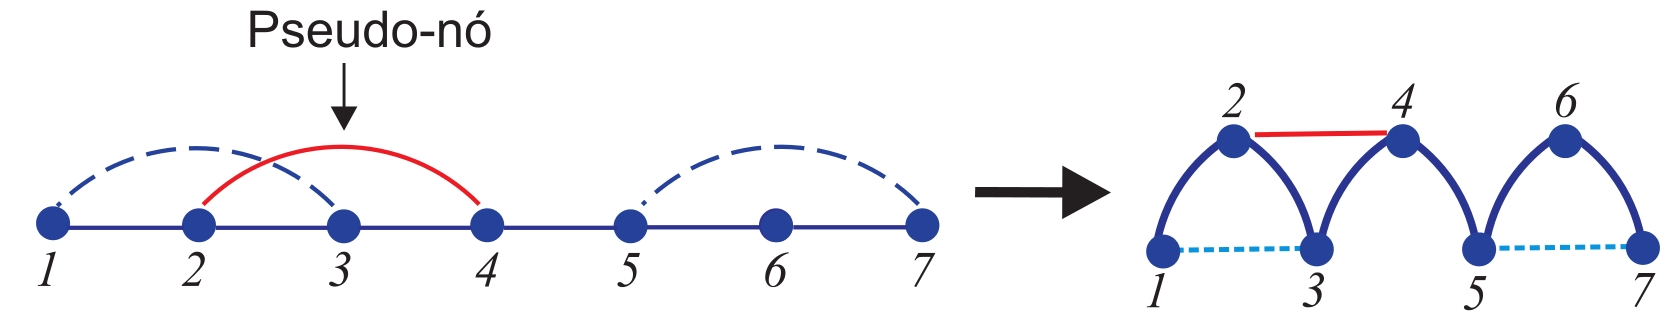
\includegraphics[angle=0,width=1.0\textwidth]{imagens//pseudono.jpg}
%\caption{Pseudo-nó (arco com linha contínua)
% - Um pseudo-nó do RNA consiste em
%um par de bases não aninhadas entre um laço de uma haste e resíduos fora desta haste
%~\citep{eddy2004rna:2004}. \label{fig:pseudono}}
%\end{figure}


\subsubsection{Proposta de Três Principais Abordagens}

Propomos uma classificação dos métodos computacionais para detecção de ncRNAs em três grupos~\citep{griffiths2007annotating:2007,Stadler:2011}:


\textbf{Homologia} \\


Predição de ncRNAs feita por meio de comparação de genomas entre duas ou mais espécies. Essas comparações dependem de bancos de dados curados, no sentido de que quanto melhores forem as anotações do banco melhores serão as predições~\citep{machado2008computational:2008}.

Dois genes são ditos homólogos se descendem de um ancestral comum, e possivelmente esses genes mantenham a mesma funcionalidade herdada. Sequências homólogas podem ser divididas em duas classes: ortólogas e parálogas. As ortólogas são sequências relacionadas por especiação, possuindo uma descendência vertical, já as parálogas são sequências relacionadas por duplicação dentro da mesma espécie ou nos ancestrais~\citep{stryer:2002}.




Duas ferramentas importantes para inferir homologia que usam como métrica similaridade de sequências (quanto maior a similaridade entre duas sequências, maior a chance delas terem herdado a mesma função) são: BLAST~\citep{altschul1990basic:1990}, uma ferramenta para detecção de ncRNAs baseada em alinhamento par a par  entre as estruturas primárias das sequências; e o Infernal~\citep{altschul1990basic:1990}, uma ferramenta baseada em alinhamento múltiplo que considera as estruturas secundárias das sequências. O BLAST em geral não produz bons resultados, sendo O Infernal mais sensível e específico para pesquisar ncRNAs~\citep{eddy2003infernal:2003}.\\


%Duas ferramentas importantes para tentar identificar a homologia por similaridade de sequências, ou seja, quanto maior a similaridade entre duas sequências, maior a chance delas terem herdado a mesma função, são o BLAST~\citep{altschul1990basic:1990}, uma ferramenta para detecção de ncRNAs baseadas em homologia que considera as estruturas primárias das sequências; e o Infernal ~\citep{altschul1990basic:1990}, que considera as estruturas secundárias das sequências. O BLAST, em geral não produz bons resultados para detecção de ncRNAs. O Infernal é mais sensível e específico para pesquisar ncRNAs~\citep{eddy2003infernal:2003}.\\

 %principais que representam a homologia são o BLAST~\citep{altschul1990basic:1990}, embora ele considere a estrutura primária da sequência; e o Infernal ~\citep{altschul1990basic:1990}, o BLAST não produz bons resultados para buscar por RNAs homólogos em bases de dados de sequências de ácidos nucléicos. O Infernal é mais sensível e específica para pesquisa de RNAs homólogos~\citep{eddy2003infernal:2003}.\\


\textbf{Predição de Classe} \\

Predição de ncRNAs feita por métodos de aprendizagem de máquina.

No aprendizado supervisionado, pode-se tomar um conjunto conhecido de ncRNAs e um conjunto conhecido de proteínas, calculando características {\it ab initio} dessas sequências, visando criar um modelo de predição de ncRNAs. Isso confere ao modelo maior confiabilidade.

Por exemplo, o SVM-PORTRAIT~\citep{Arrial:2006,arrial2009screening:2009} mostra um grau de acurácia elevado para sequências de transcritomas ainda não totalmente caracterizadas.\\


%Por exemplo, no aprendizado supervisionado toma-se um conjunto conhecido de ncRNAs, e um conjunto conhecido de proteínas das sequências, a predição de ncRNAs pode ser feita com maior confiabilidade, e usando \textit{ab initio}. Por exemplo, o SVM-PORTRAIT~\citep{Arrial:2006} que mostra um grau de acurácia elevado.\\




% sua estrutura secundária pode ser predita com maior confiabilidade, pois conservação de domínios estruturais em diferentes espécies constitui evidência adicional de que esses domínios estão relacionados com a função específica destas sequências. Com isso, estruturas conservadas são úteis para descobrir e caracterizar assinaturas de uma família específica de RNAs, e podem ser utilizadas para classificar um RNA como membro de uma família comparando sua estrutura com a estrutura das várias famílias conhecidas.

%Métodos que utilizam aprendizado de máquina mostraram um grau de acurácia elevado, como o SVM-PORTRAIT~\citep{Arrial:2006}. \\


\textbf{Modelos \textit{De Novo}} \\

Predição de nRNAs feita por outros modelos, diferentes de {\it homologia} e {\it predição de classe}.

Por exemplo, no modelo termodinâmico, a composição e ordenação de nucleotídeos em uma molécula de RNA é responsável por sua conformação espacial. Uma investigação dessa conformação, por sua vez, resulta em um conhecimento aproximado tanto sobre a organização da molécula quanto sobre suas propriedades fisiológicas. A avaliação termodinâmica de moléculas de RNA pode ser utilizada em conjunto com regras estruturais e topológicas para inferir a estrutura secundária ativa da molécula de RNA~\citep{zuker1981optimal:1981}. 


Um RNA com uma estrutura secundária bem definida tem energia livre associada menor do que sequências com a mesma frequência de nucleotídeos, porém sem estrutura secundária definida~\citep{machado2008computational:2008}. A partir da análise da energia livre mínima de uma molécula de RNA, é possível inferir se ela tem uma conformação de estrutura secundária estável.


%O modelo \textit{De Novo}~\citep{griffiths2007annotating:2007} (inclui outros modelos, como o termodinâmico) pesquisas em transcritômica tem se beneficiado imensamente com o advento das estratégias de sequenciamento de alto desempenho. Sem a necessidade do emprego de técnicas de clonagem, as modernas plataformas  comerciais de sequenciamento podem sequenciar diretamente DNA complementar (cDNA) ou o RNA mensageiro (RNAm) em larga escala.

%Com isso novos algoritmos e técnicas são necessários para analisar e
%classificar as sequências geradas pelas novas plataformas de sequenciamento, 
%surgindo assim o \textit{De Novo}, que tem como objetivo melhorar a acurácia
%e diminuir as deficiências dos métodos anteriores. 
